\chapter{Montagem do projeto}
Neste capítulo serão comentados os procedimentos adotados para a montagem do projeto do regulador de temperaturas, como o circuito implementado na protoboard e as conexões na parte interna do chuveiro.

\section{Circuito de controle de temperatura}

O circuito microcontrolado para testes foi montado e testado em um dos laboratórios do Núcleo de Pesquisa e Desenvolvimento em Engenharia Elétrica (NUPEDEE) localizado na Universidade Federal de Santa Maria. Na figura abaixo podemos ver o circuito implementado em uma protoboard.

\begin{figure}[H]

\center

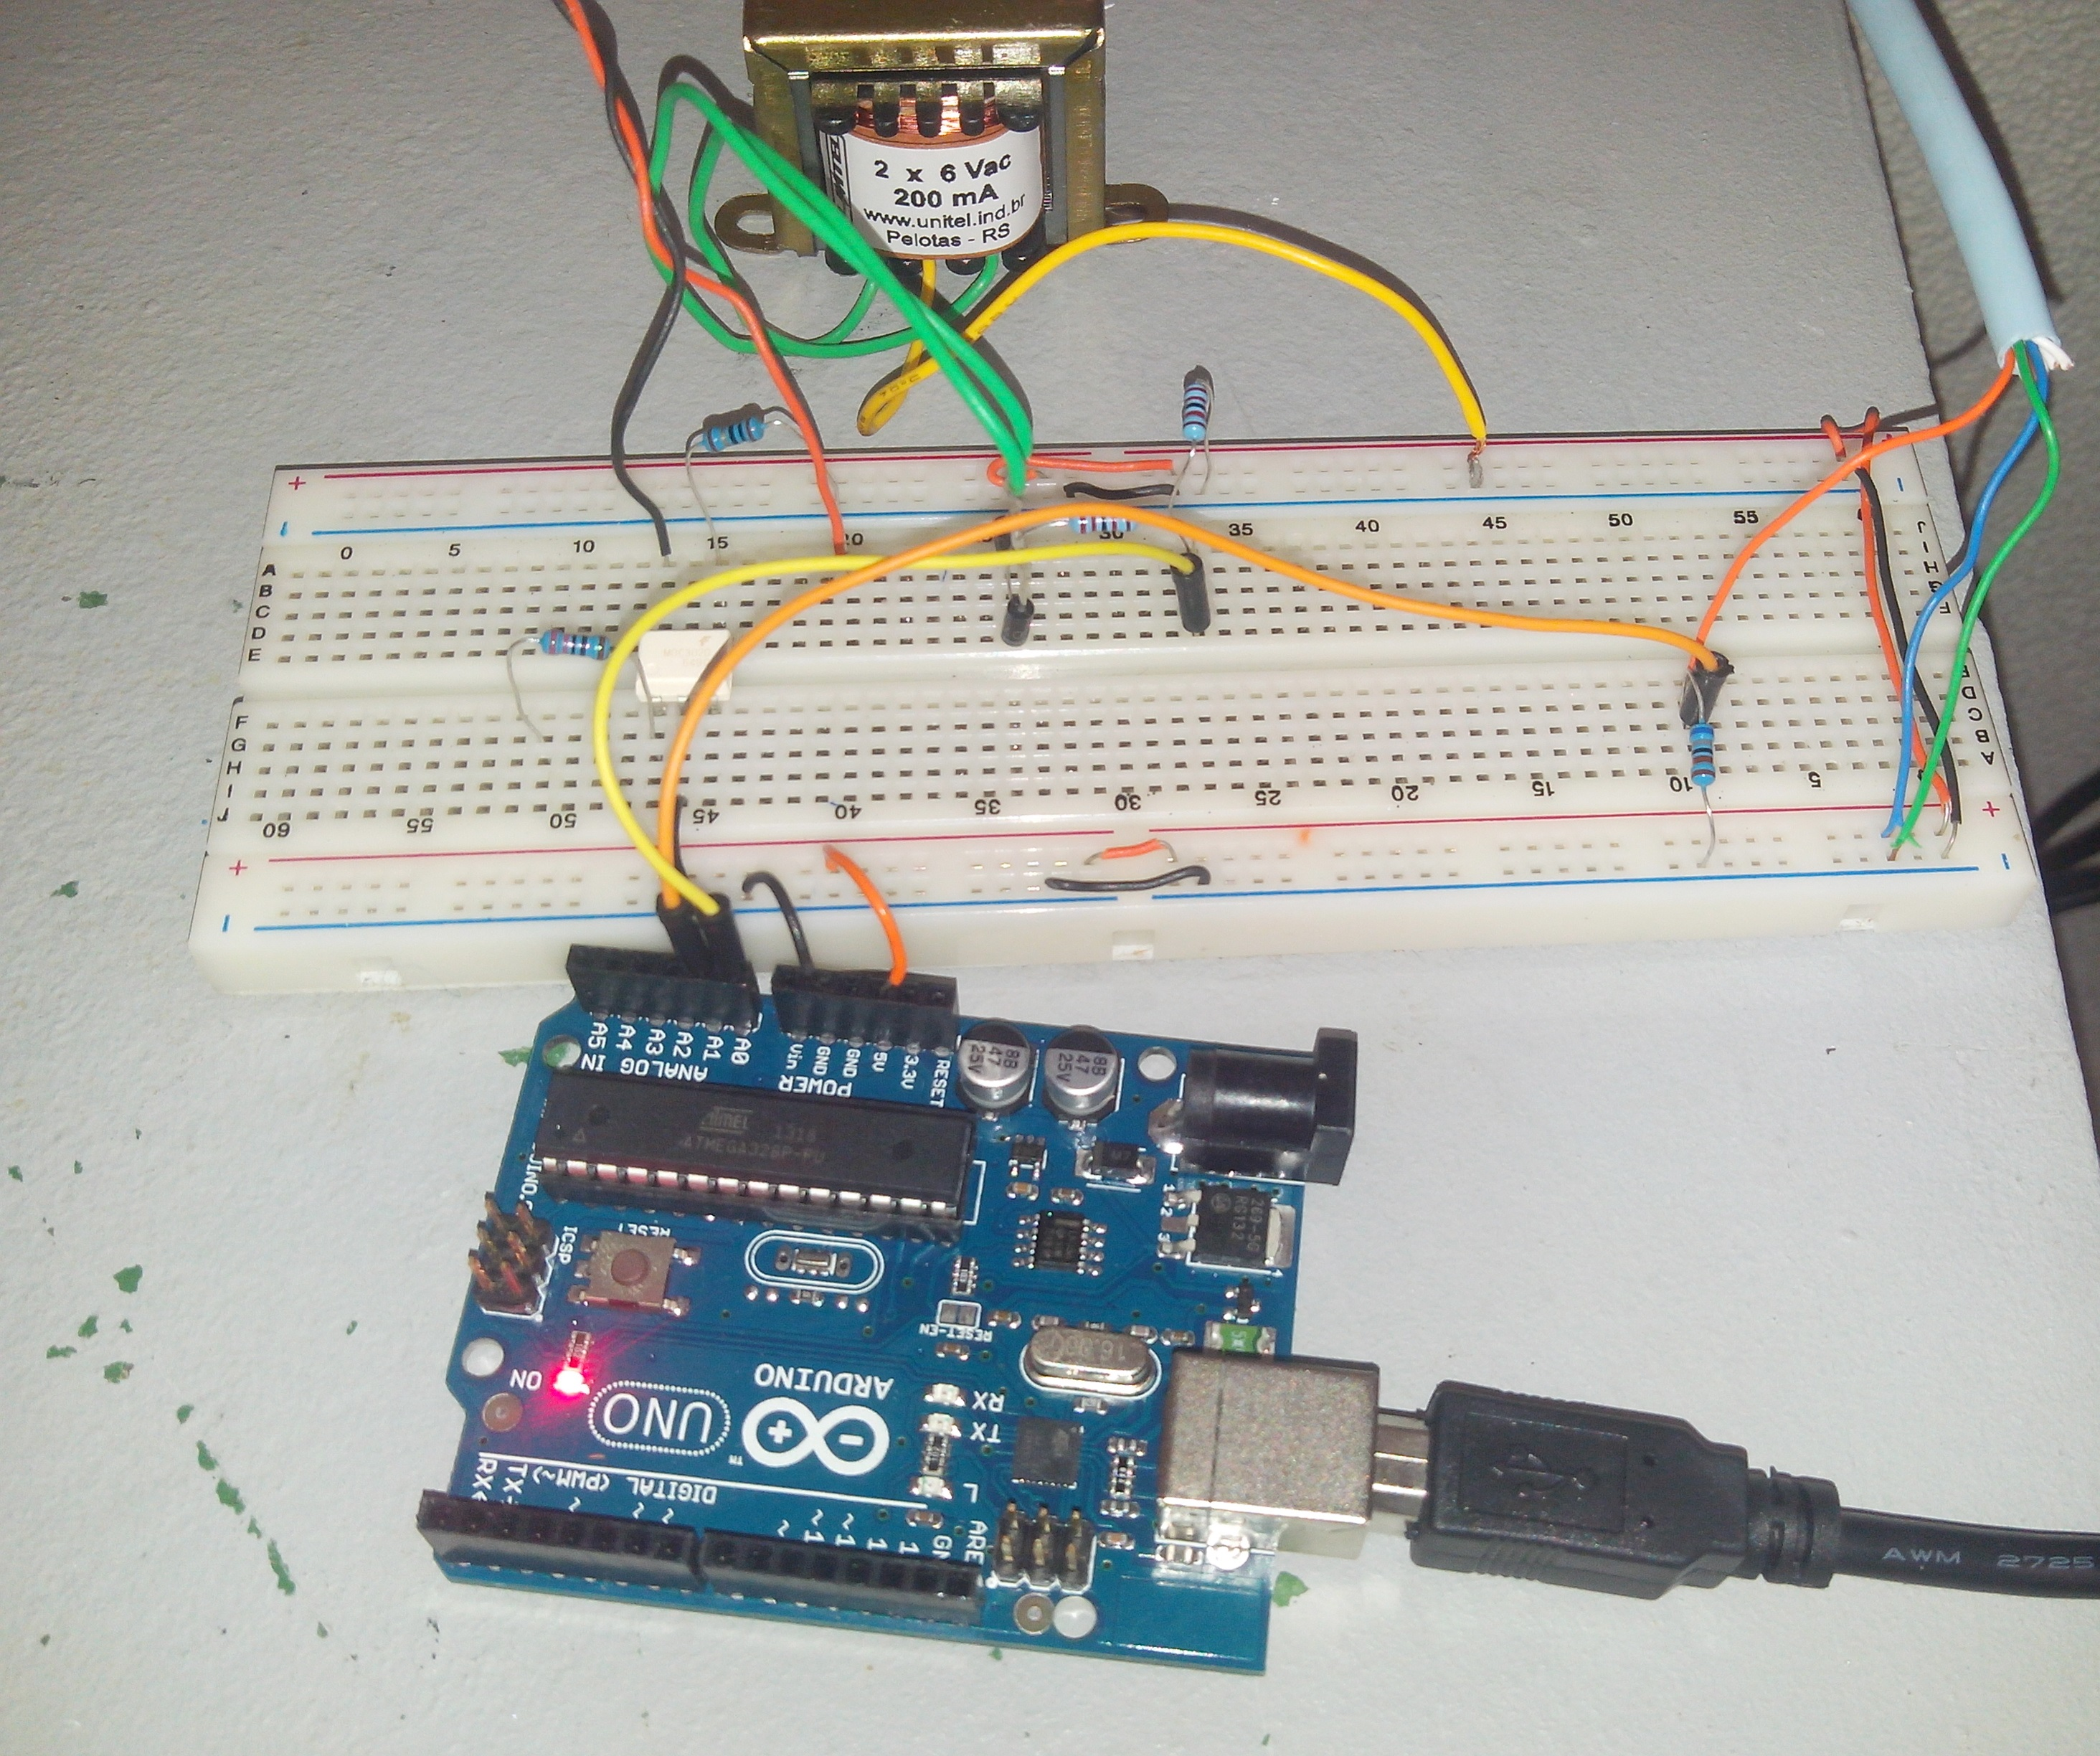
\includegraphics[width=10cm]{imagens/circuito_testes.jpg}

\label{Teste do circuito de controle}

\caption{Teste do circuito de controle}

\end{figure}

\section{Instalação no chuveiro}
Primeiramente a ducha ThermoSystem foi desmontada retirando-se o circuito de controle de temperatura convencional, cujo funcionamento foi comentado no capítulo 3. Após a retirada, foram soldados quatro fios no circuito interno do chuveiro. A tabela 4.2 representa as conexões dos fios soldados ao circuito microcontrolado.

\begin{table}[!hbt] 
   \centering   % tabela centralizada
   \setlength{\arrayrulewidth}{1\arrayrulewidth}
   \setlength{\belowcaptionskip}{5pt}
   
   \renewcommand{\arraystretch}{2}
   
   \caption{Conexões do chuveiro ao circuito microcontrado}
   \begin{tabular}{|l|l|} % c=center, l=left, r=right 
      \hline
      \textbf{Fio} &\textbf{Conexão} \\
      \hline 
      MT2 (TRIAC) & Terminal 4 do optoacoplador \\ 
     \hline
      \textit{Gate} (TRIAC) & Terminal 6 do optoacoplador \\
      \hline 
      Fase da rede & Alimentação do Transformador \\  
      \hline 
      Neutro da rede &	Neutro do transformador\\
      \hline
   \end{tabular}
   \label{Conexões do chuveiro ao circuito microcontrado}
\end{table}

O MT2 conectado ao terminal 4 do optoacoplador terá a função de disparar o TRIAC após o microcontrolador realizar a detecção de passagem por zero e calcular a lei de controle do sistema. A fase e o neutro da rede são conectados ao transformador que só irá conduzir corrente elétrica quando houver passagem de água pelo diafragma (abertura do registro) fazendo com que dois contatos se encostem fechando a malha do circuito. A figura 4.2 mostra as conexões dos fios na parte interna do chuveiro.

\begin{figure}[H]

\center

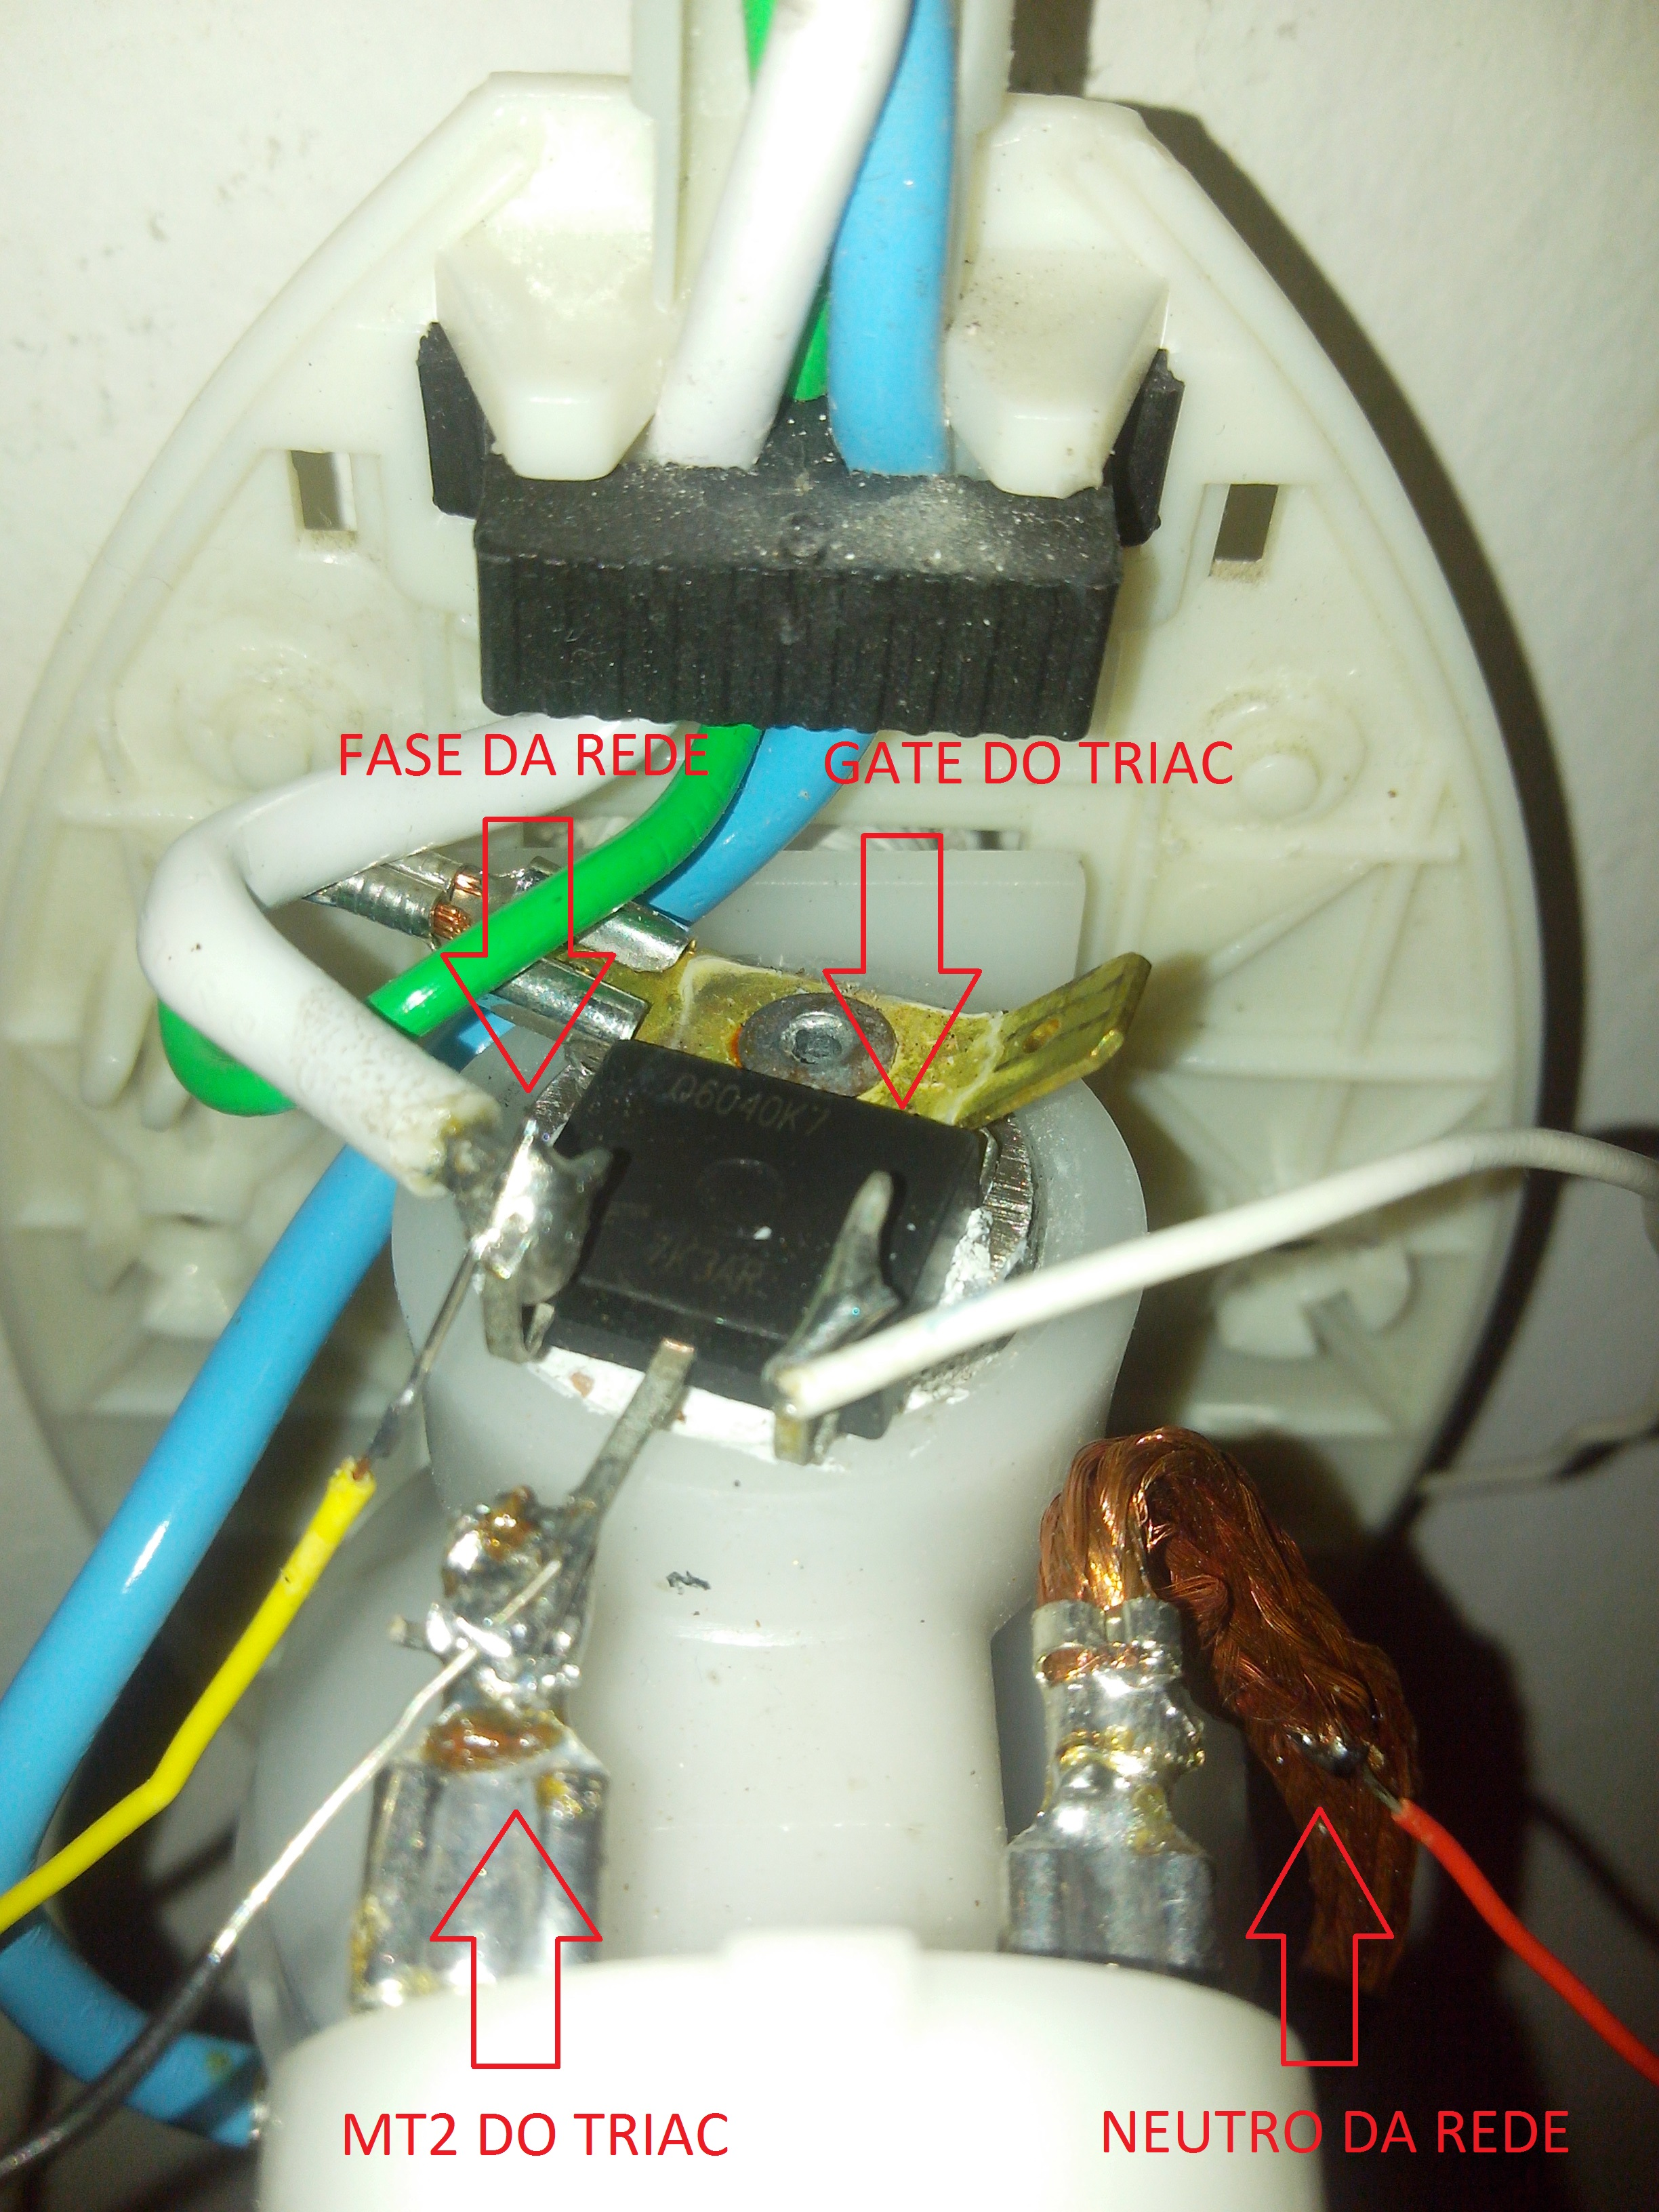
\includegraphics[width=7cm]{imagens/Chuveiro_INTERNO.jpg}

\label{Conexões da parte interna do chuveiro}

\caption{Conexões da parte interna do chuveiro}

\end{figure}

Após a instalação na parte interior do chuveiro, foi realizada a instalação do sensor de temperatura. Ele foi posicionado abaixo da saída de água do espalhador para que a água ao passar por ele aqueça-o gerando assim um sinal analógico na saída do sensor referente a temperatura e possibilitando a leitura deste sinal na porta analógica do microcontrolador.Seus terminais foram conectados a protoboard que, por sua vez, foram conectado aos devidos pinos do Arduino. A figura 4.3 mostra como foi realizada a instalação do sensor de temperatura.

%placa de circuito impresso que contem o microcontrolador ATmega328 e alguns componentes eletrônicos
%protoboard que, por sua vez, foram conectado aos devidos pinos do Arduino.

\begin{figure}[H]

\center

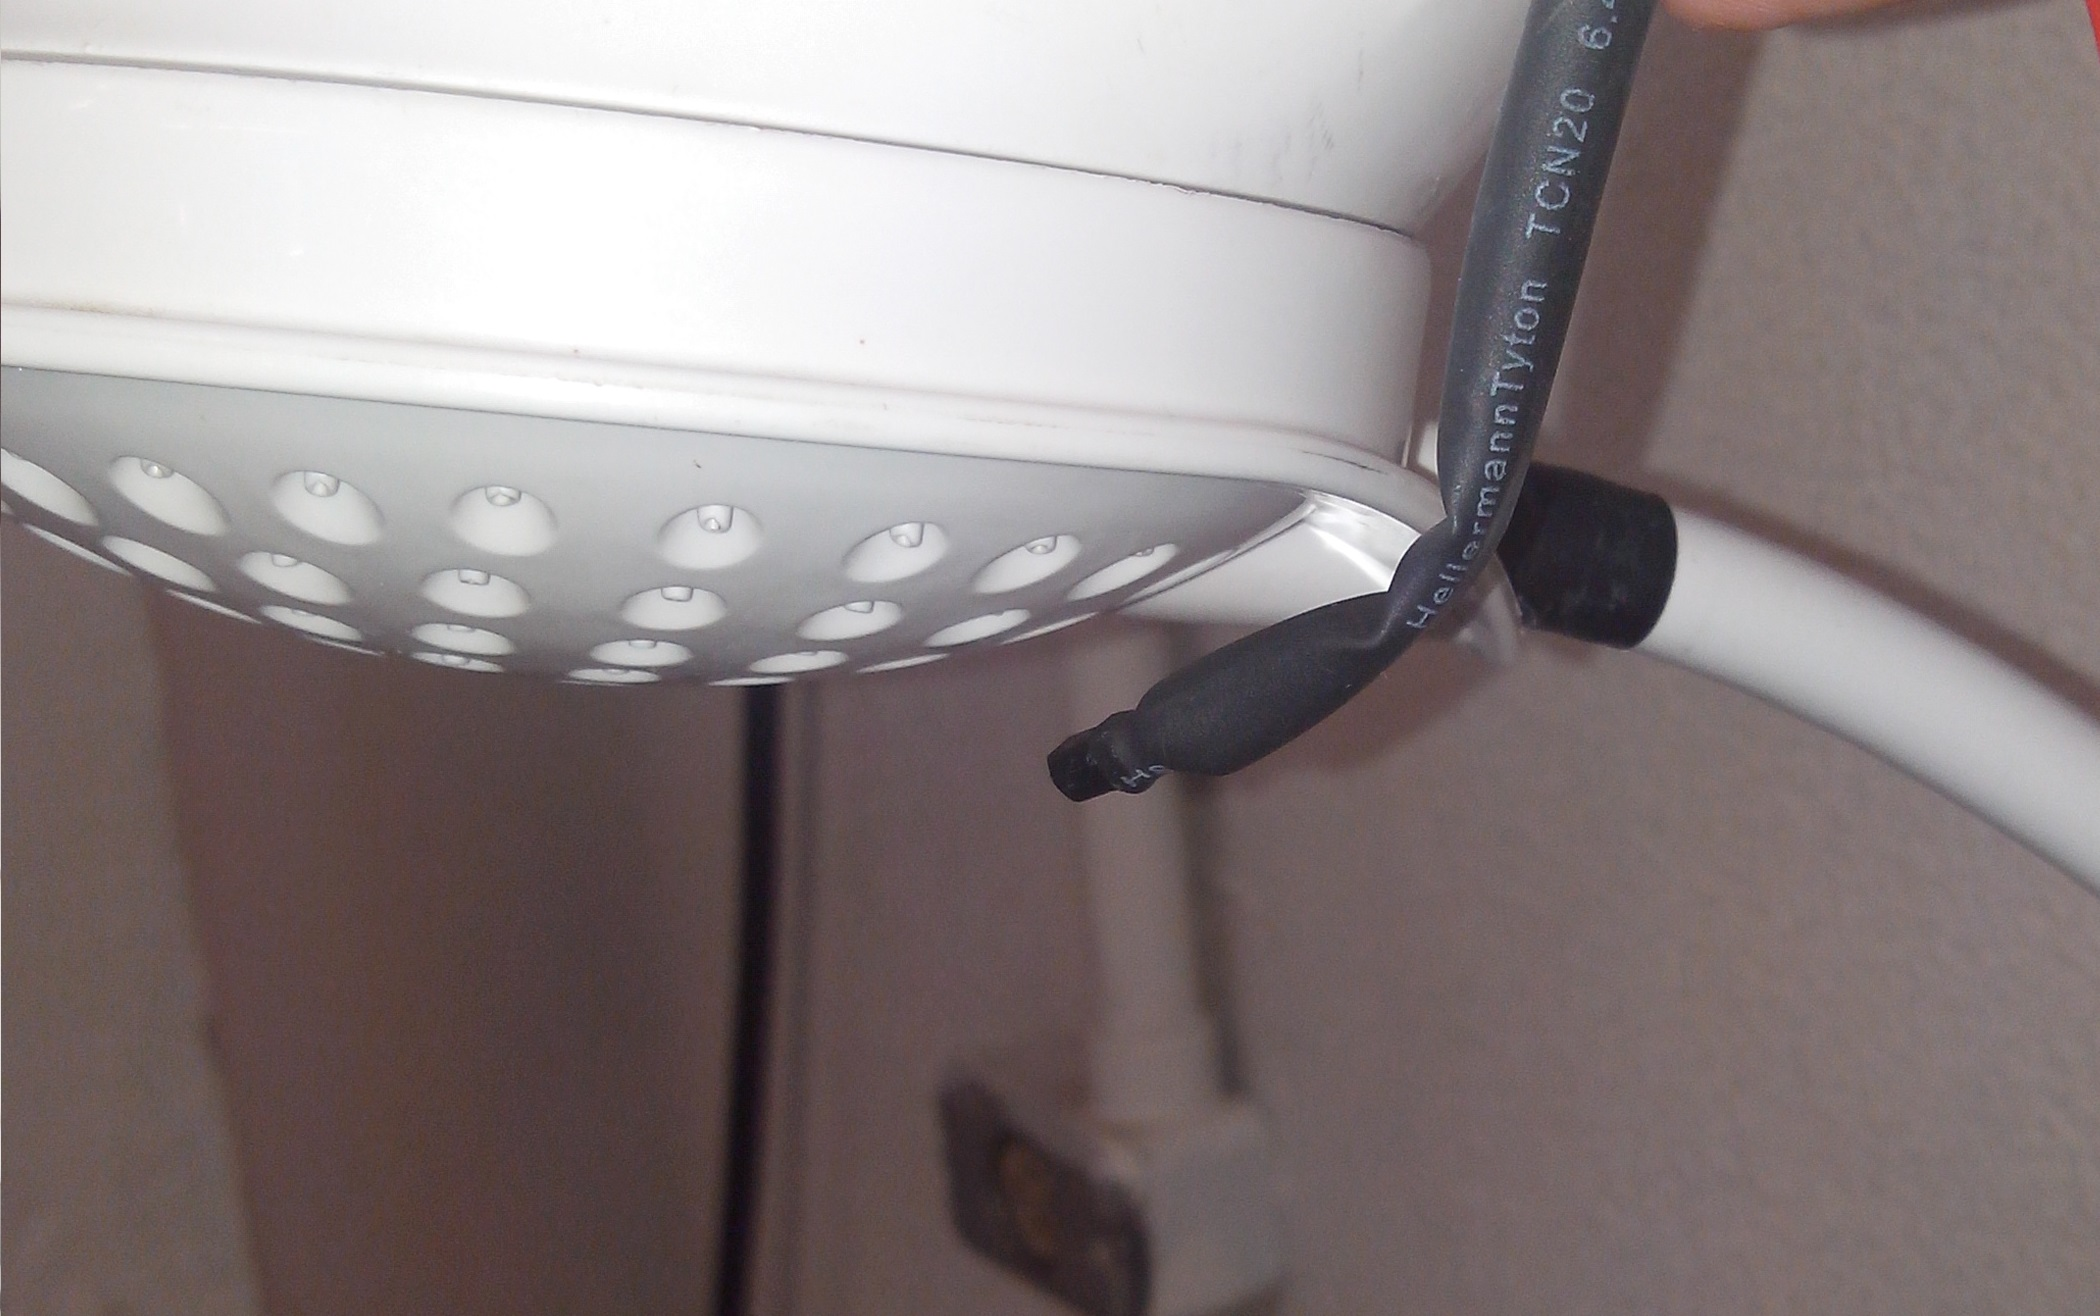
\includegraphics[width=9cm]{imagens/sensor_espalhador.jpg}

\label{Instalação do sensor de temperatura}

\caption{Instalação do sensor de temperatura}

\end{figure}


\section{Implementação no microcontrolador}

Os cálculos das leis de controle aplicadas ao sistema para que ele atinja a estabilidade são realizados toda vez que há a passagem por zero Volt na porta analógica do microcontrolador e são aplicados apenas no próximo ciclo.
O fluxograma mostrado na figura 4.4 representa a lógica do sistema.

\begin{figure}[H]

\center

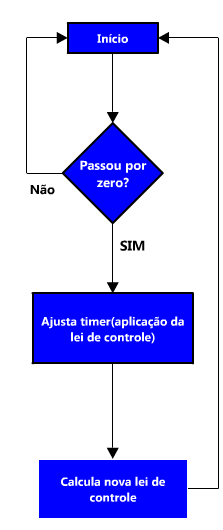
\includegraphics[width=4cm]{imagens/fluxograma_controle.png}

\label{Lógica do sistema}

\caption{Lógica do sistema}

\end{figure}

\section{Circuito Impresso}

Após serem realizados os testes de estabilidade do sistema, a implementação da interface e do circuito de controle foram desenvolvidas na ferramenta CAD chamada \textit{Eagle}.

A placa da interface do circuito possui dois displays de sete segmentos e dois botões. Os displays tem a função de mostrar a temperatura desejada da água, enquanto os botões tem a função de incrementar ou decrementar essa temperatura. As figuras 4.5 e 4.6 mostram respectivamente o esquemático da placa no \textit{Eagle} e a placa já impressa com seus componentes soldados.

\begin{figure}[H]

\center

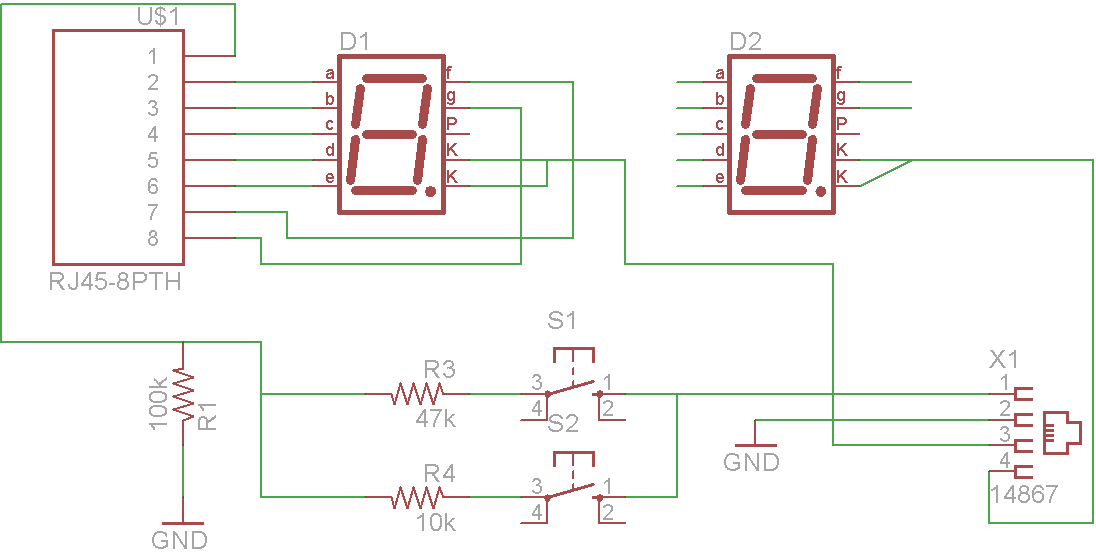
\includegraphics[width=12cm]{imagens/projeto_interface.png}

\label{Esquemático da placa de interface}

\caption{Esquemático da placa de interface}

\end{figure}


\begin{figure}[H]

\center

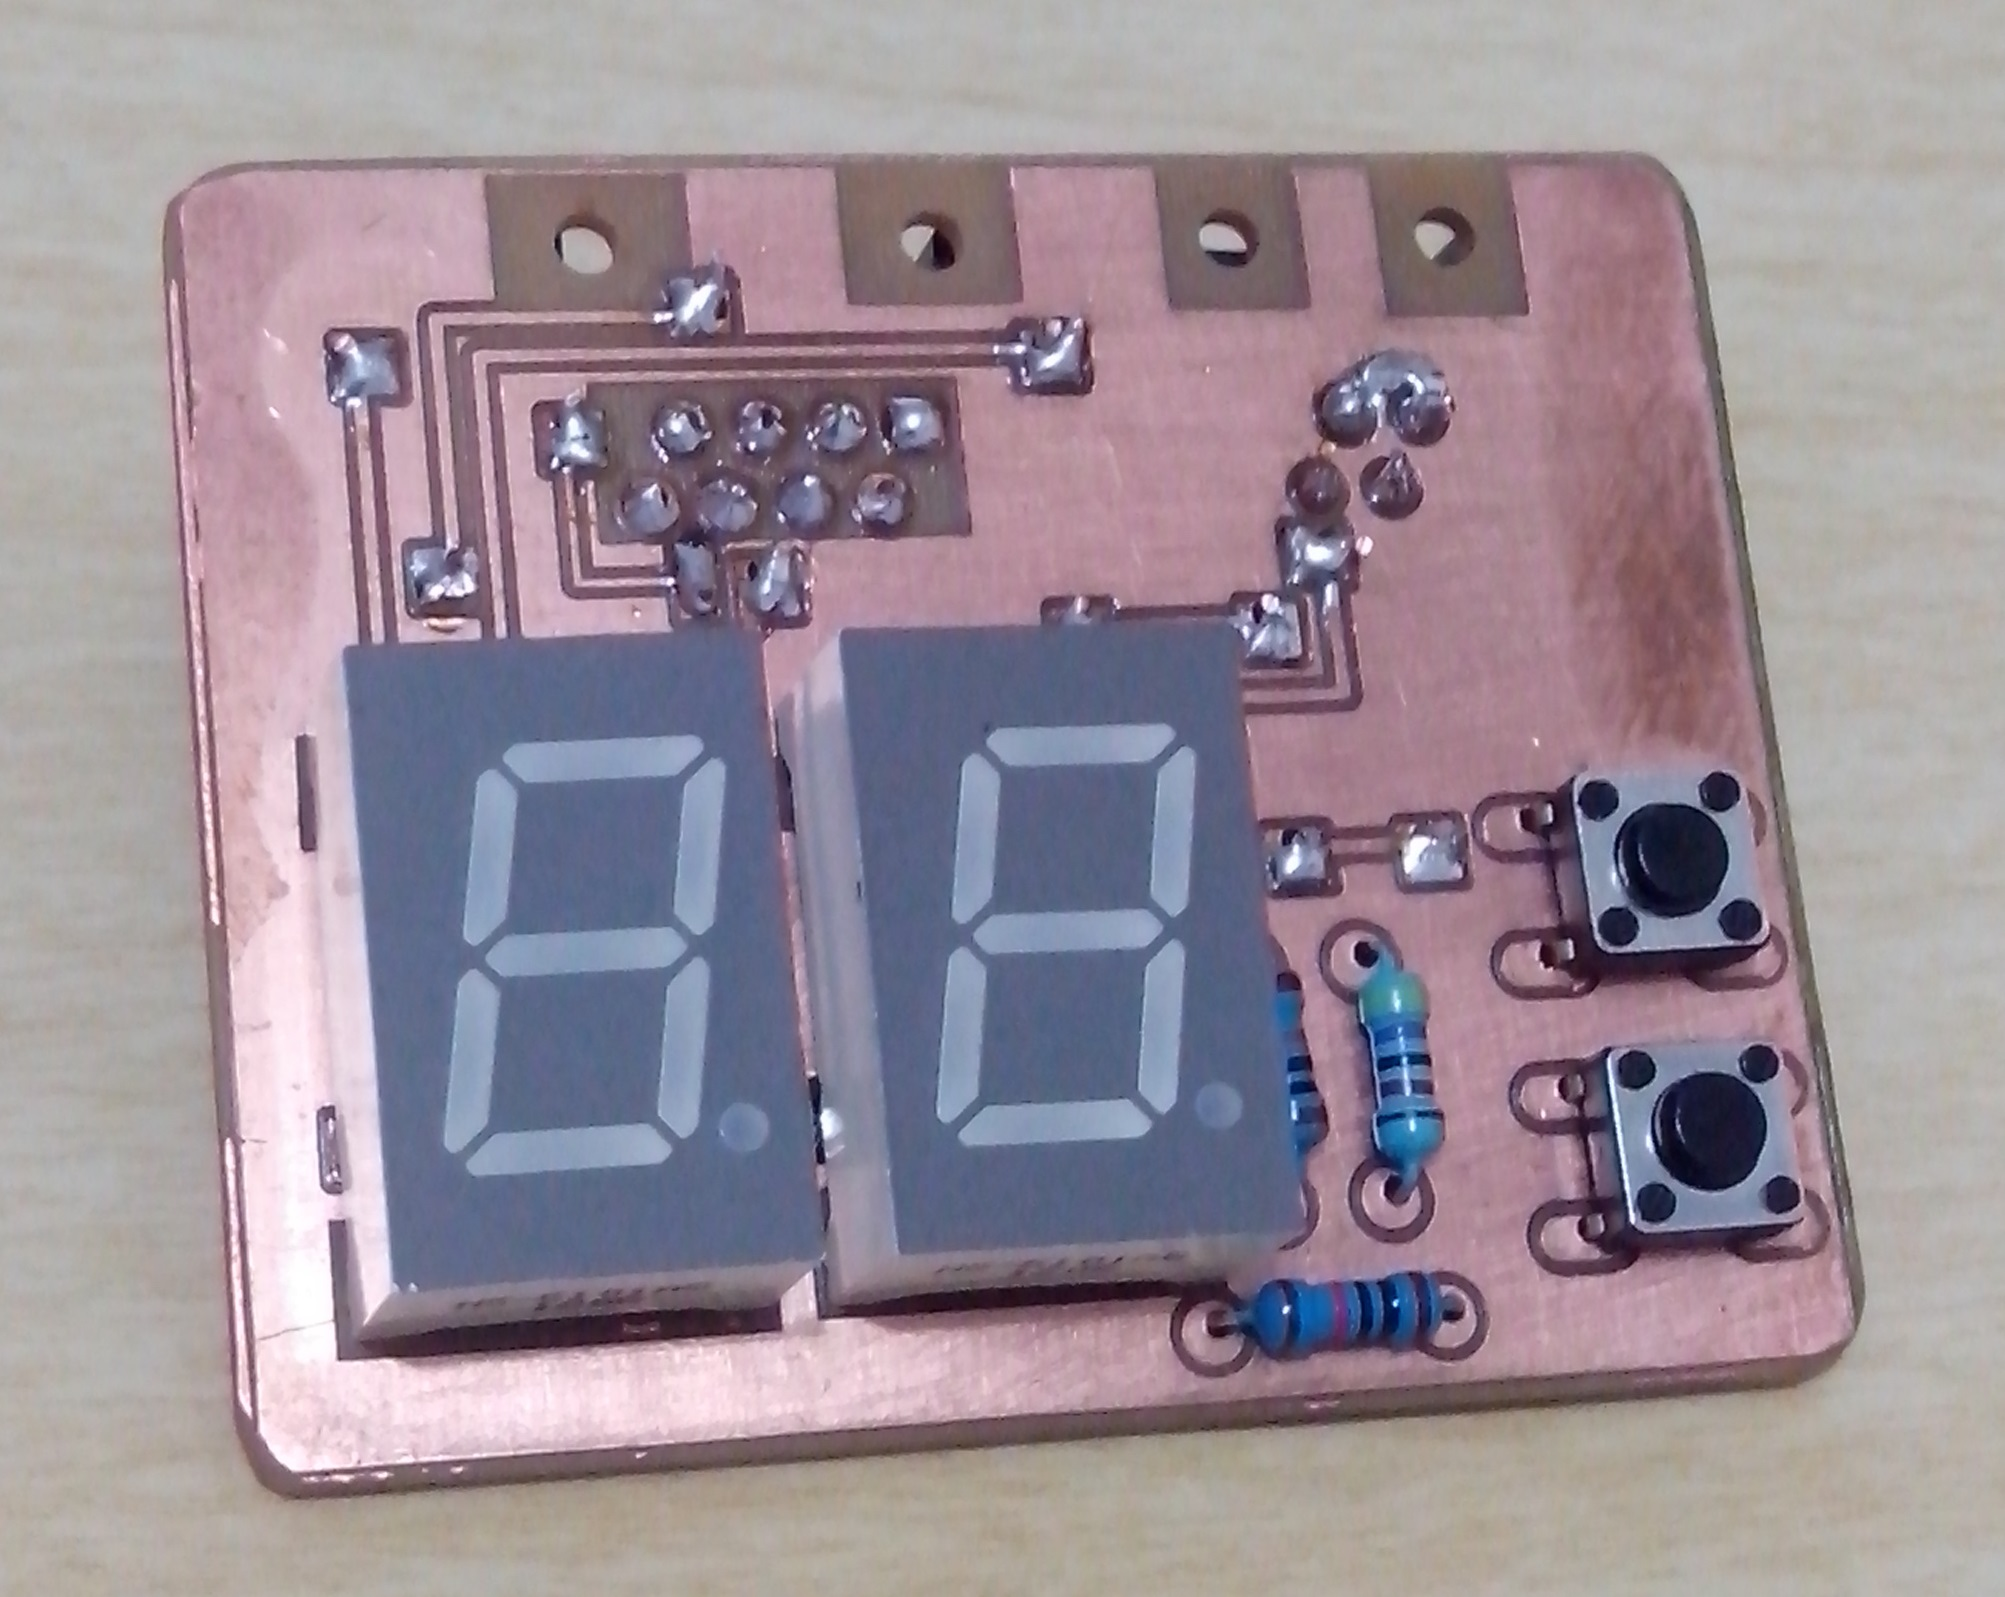
\includegraphics[width=10cm]{imagens/placa_interface.jpg}

\label{Placa de interface}

\caption{Placa de interface}

\end{figure}



A placa do circuito de controle possui um microcontrolador ATmega328, um optoacoplador, componentes eletrônicos como resistores, capacitores, diodos e transistores e um regulador de tensão. Esta placa terá a funcão de substituir a plataforma de prototipagem (Arduino UNO), e realizar todo o controle do sistema. Sua localização será na parte interna do chuveiro. As figuras 4.7 e 4.8 mostram respectivamente o esquemático do circuito de controle e a placa impressa com os componentes.

\begin{figure}[H]

\center

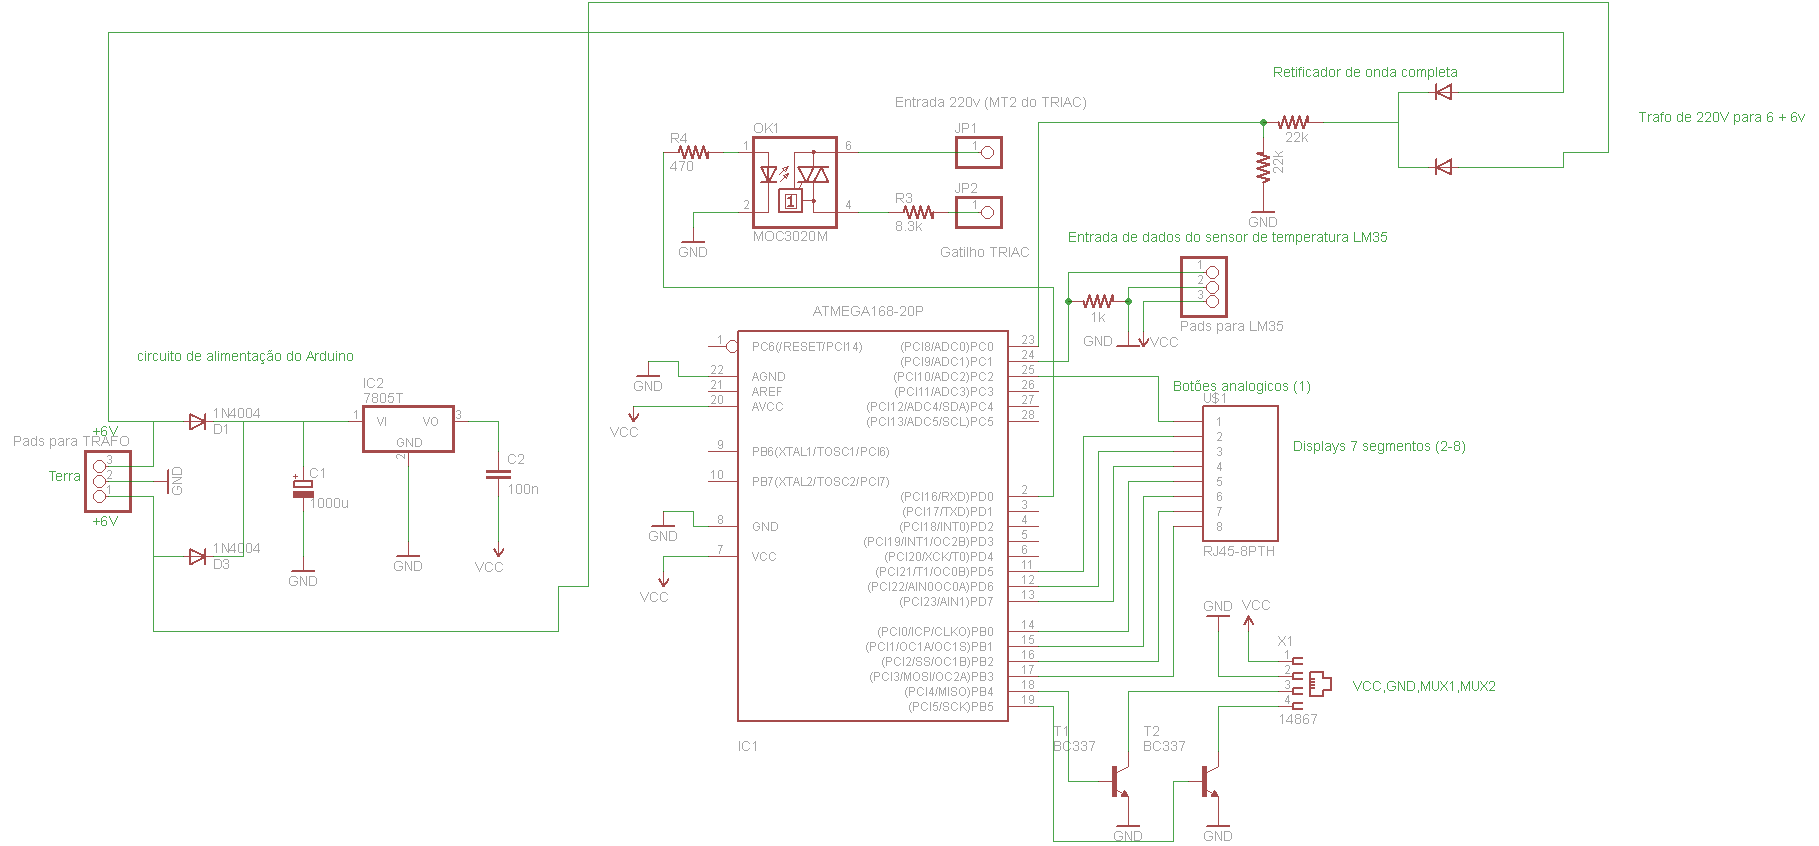
\includegraphics[width=15cm]{imagens/projeto_controle.png}

\label{Esquemático do circuito de controle}

\caption{Esquemático do circuito de controle}

\end{figure}

\begin{figure}[H]

\center

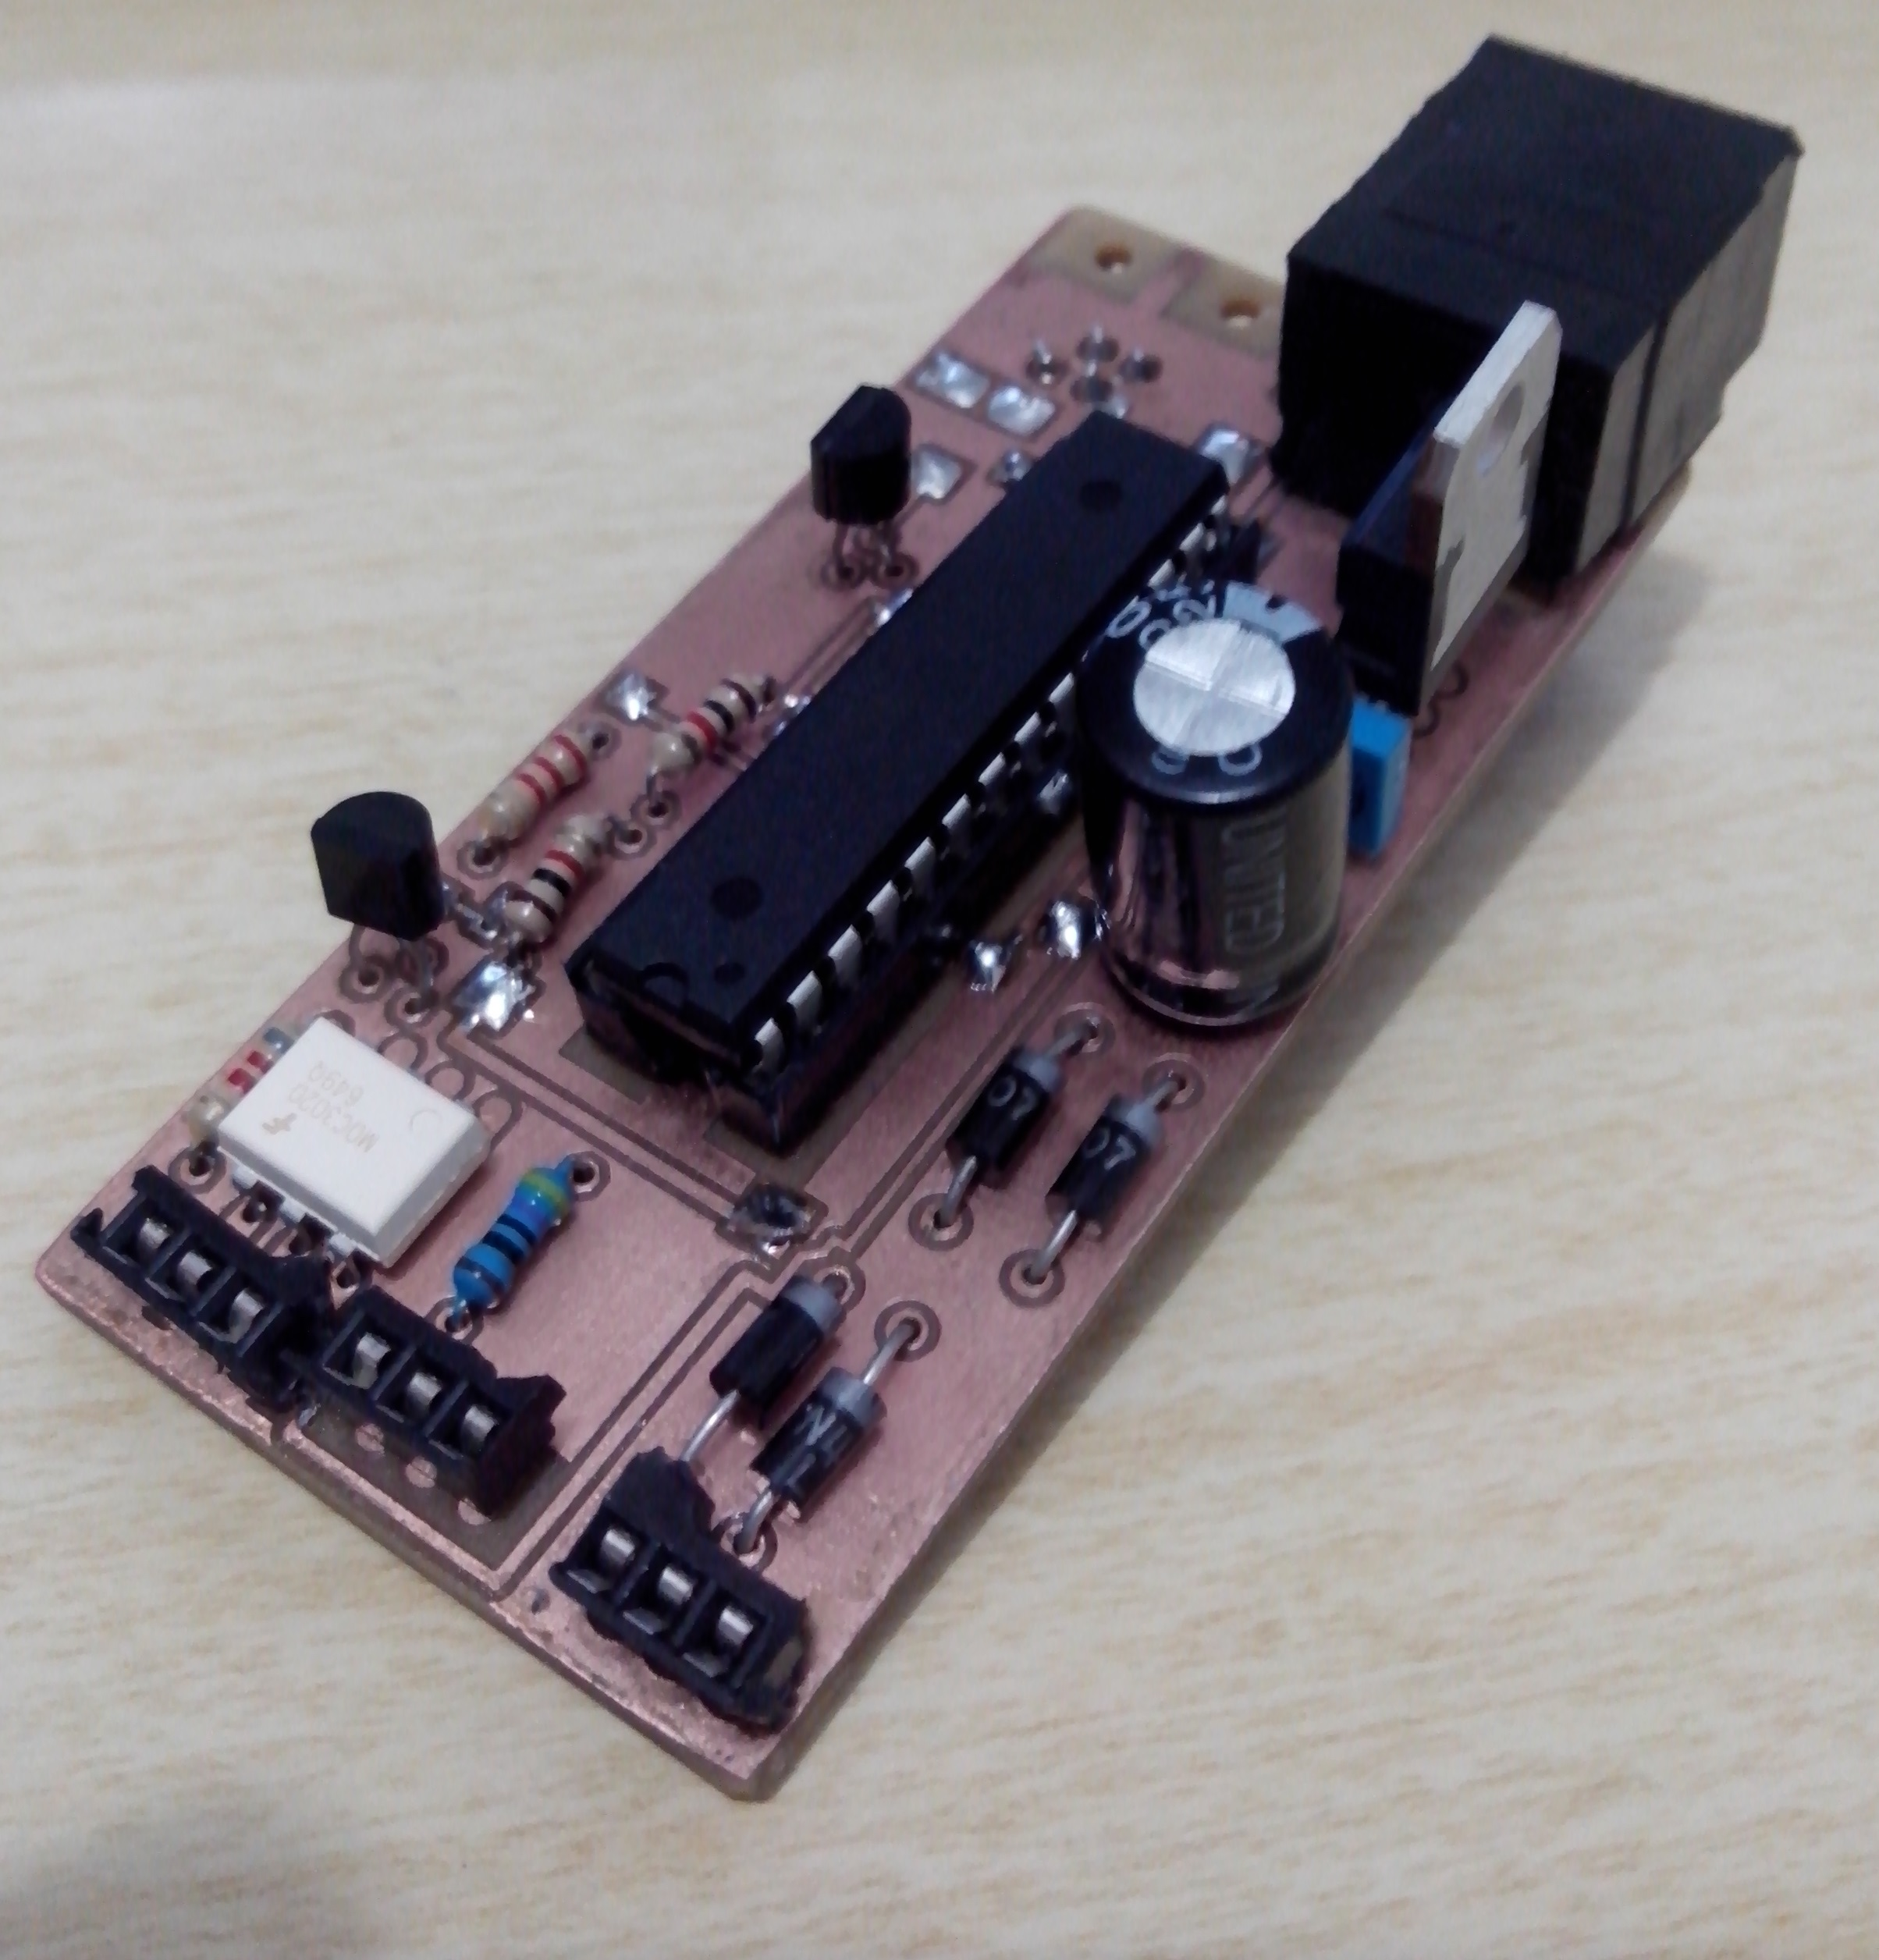
\includegraphics[width=10cm]{imagens/circuito_microcontrolado.jpg}

\label{Circuito de controle}

\caption{Circuito de controle}

\end{figure}
